\documentclass[12pt]{report}

% font style
\usepackage[utf8]{inputenc}
\usepackage[T1]{fontenc}
\usepackage{mathptmx}
\usepackage[fontsize=13pt]{scrextend}

% code
\usepackage{listings}
\usepackage{color}

\definecolor{dkgreen}{rgb}{0,0.6,0}
\definecolor{gray}{rgb}{0.5,0.5,0.5}
\definecolor{mauve}{rgb}{0.58,0,0.82}

\lstset{frame=tb,
  language=Java,
  aboveskip=3mm,
  belowskip=3mm,
  showstringspaces=false,
  columns=flexible,
  basicstyle={\small\ttfamily},
  numbers=none,
  numberstyle=\tiny\color{gray},
  keywordstyle=\color{blue},
  commentstyle=\color{dkgreen},
  stringstyle=\color{mauve},
  breaklines=true,
  breakatwhitespace=true,
  tabsize=3
}

\usepackage{graphicx}
\usepackage[a4paper,left=25mm,right=25mm,top=25mm,bottom=25mm]{geometry}
\usepackage{fancyhdr}
\usepackage{caption}
\usepackage{subcaption}
\pagestyle{fancy}
\fancyhead{}
% \fancyhead[RO,LE]{Apply neural network in EEG signal processing}
\fancyhead[RO,LE]{Characterization of EEG signals according to brain regions using machine learning techniques}
\fancyfoot{}
\fancyfoot[LE,RO]{\thepage}
\fancyfoot[LO,CE]{Chapter \thechapter}
\fancyfoot[CO,RE]{Lai Khang Duy}
\renewcommand{\headrulewidth}{0.4pt}
\renewcommand{\footrulewidth}{0.4pt}

%\usepackage[style=authoryear,sorting=none]{biblatex}
%\addbibresource{1.bib}

\graphicspath{{images/}}

\title{
	{Characterization of EEG signals according to brain regions using machine learning techniques}\\
	{\large University of Science and Technology of Hanoi}\\
	{\large Technical University of Ostrava}
	\bigskip
	\\
	{
\includegraphics[scale=0.5]{logo2.png}   
\includegraphics[scale=0.4]{download.png}}
}

\author{{Lai Khang Duy}
		\bigskip
		\\
		{External supervisor: Prof. Sebastián Basterrech}\\
		{Internal supervisor: Prof. Nghiem Thi Phuong}
}
\date{\large August 16 2019}


\begin{document}
	
\maketitle

\tableofcontents

\chapter*{Acknowledgements}

First and foremost, I would like to express my gratefulness and sincerely to my supervisor, Professor Sebastián Basterrech, for giving me a wonderful opportunity to work and study in this machine learning topic, for the continuous support me during my internship in the Czech Republic and for his patience, motivation and immense knowledge. His guidance helps me to follow the correct path in the time I worked. I could not have imagined having a better supervisor and mentor in my very last and important time to finish the Bachelor program outside of my home country.

My sincere also goes to my extraordinary internal supervisor, Prof. Nghiem Thi Phuong, who do not hesitate to help me anything, especially help me to finish my papers with University of Sciences and Technologies of Hanoi and the Czech Republic Embassy. I will unable to have this nice and remarkable internship without her.

I would like to show my thankfulness to all my teachers, who have been along side with me in three years at University of Sciences and Technologies of Hanoi. It is a great pleasure to be your student.

I would like also to give the great respect to Technical University of Ostrava, that provide me a place to live, a place to work, and the equipment that I use during the internship, my very kind roommate Vo Gia Thinh, as well as my labmate, Radek, Sue Lei and Ling Ping, to help me on the very first day I came to Ostrava.

Last but not least, I want to give a great gratefulness to my family for giving me a lot of mental as well as financial support. This thesis could not be here without them.

     
\chapter*{Declaration}
I hereby declare that this bachelor thesis was written by myself. I have quoted all the references I have drawn upon.\\
The work was done under the guidance of Professor Sebastián Basterrech, at Faculty of Electrical and Information, Technical University of Ostrava.\\

\bigskip
Lai Khang Duy

Ostrava, July 30, 2019
     

\listoffigures

% \listoftables

\chapter*{List of acronyms}
    \begin{itemize}
        \item USTH: University of Science and Technology of Hanoi
        \item VSB: Technical University of Ostrava
        \item EEG: Electroencephalography
        \item EOG: Electrooculography
        \item ECG: Electrocardiography
        \item RNN: Recursive neural network
        \item LSTM: Long short-term memory
        \item SVM: Support vector machine
    \end{itemize}

\chapter*{Abstract}
Almost any living creatures on the planet have brains. Brain is the most complex organ that exist in a living body and act a highly important role in the activities. When the brain is working and neurons transmit signal to each other, it generates electrical signals. With our technology today, we can measure the strength of the signal to analysis the body's behavior. This technique is called electroencephalography. However, each region of the brain is working on different tasks, which leads to the fact that the signal we measure over electrodes can really differentiate. In several cases, we need to classify the signal we measured belong to which part of the brain. In this article, I will apply both well-known machine learning techniques, recursive neural network (RNN) with long short-term memory (LSTM) and support vector machine(SVM) to classify the signal to 4 different classes after denoise the dataset using Z-score. The 4 classes are corresponding to 4 regions of the brain, Frontal lobe, Cerebellum, Parietal lobe and Occipital lobe and finally Temporal lobe.

\bigskip
Keywords: electroencephalography, classification, SVM, RNN, LSTM 
     

\chapter{Introduction}
Neural activity in human's brain starts between the 17th and 23rd week of the prenatal development. It is believed that the electrical signal of the brain is not just reflecting the activity of the brain, but also the reflecting the activity of the whole body. This trust leads to the fact that people assume that if the brain signal can be recorded and analyze, scientists can further have more knowledge about the own human's body~\cite{EEGSignalProcessing}.

 Electroencephalography, or in a shorten word is EEG, is a method to record the neural oscillations (often known as "brain waves") of the brain and illustrate the operation of the body of human by that electrical signals. There are a lot of applications using this technique nowadays, mostly diagnose epilepsy, it is also used to diagnose sleep disorders and many more~\cite{EEG2}.
 
 Our objective is to characterize EEG signals according to the specific areas of the brain. We analyze the spatial-temporal patterns of the signals using machine learning tools. Given an EEG signal, the goal is to predict which part of the brain it belongs. To have such automatic tool can be very helpful for analyzing the plasticity of the brain, and useful for understanding how brain damages provoke changes in their functionality. It is known that when some area of the brain is damaged, the brain plasticity provokes that other parts can be activated and to have new functionalities in order of mitigating the impact of brain damages.

The goal of this thesis is to try and compare 2 popular machine learning techniques with different time steps to categorize 4 classes of EEG signal that provided. Each class will corresponding with a specific region of the brain.

The thesis is divided into 7 different chapters. In the second chapter, in order to have a basic idea of what and why we do this study, we will cover a theoretical background of the problem. Chapter 3 will cover the material that we use, chapter 4 and 5 is the preprocessing process and the machine method that we applied. Finally, in chapter 6 and 7, The results will be shown. We will have a conclusion and discuss about what to improve in the future.

\chapter{Theoretical background}

\section{Electroencephalography}
    \subsection{Brain electrical signal}
    Brain is an extremely important organ that exists in all vertebrates and most invertebrates that living on planet Earth. Enveloping the brain is a complex layer of cranium and the mandible as known as the skull located in the cranial cavity, usually near the other sensory organs, such as visual, auditory, gustatory, olfaction and equilibrioception. Brain is an extremely complex organ, the human brain has over 86 billion neurons, and each connects to thousands of others to create a network. This extraordinary network expresses that it is a very effective system. In order to transmit the signal between neurons over synapses at a very high speed to make its efficiency and fast connection, the signal that neural generates for contacting each other is basically nothing else but electrical signal.
    
        \begin{figure}[h]
        \centering
        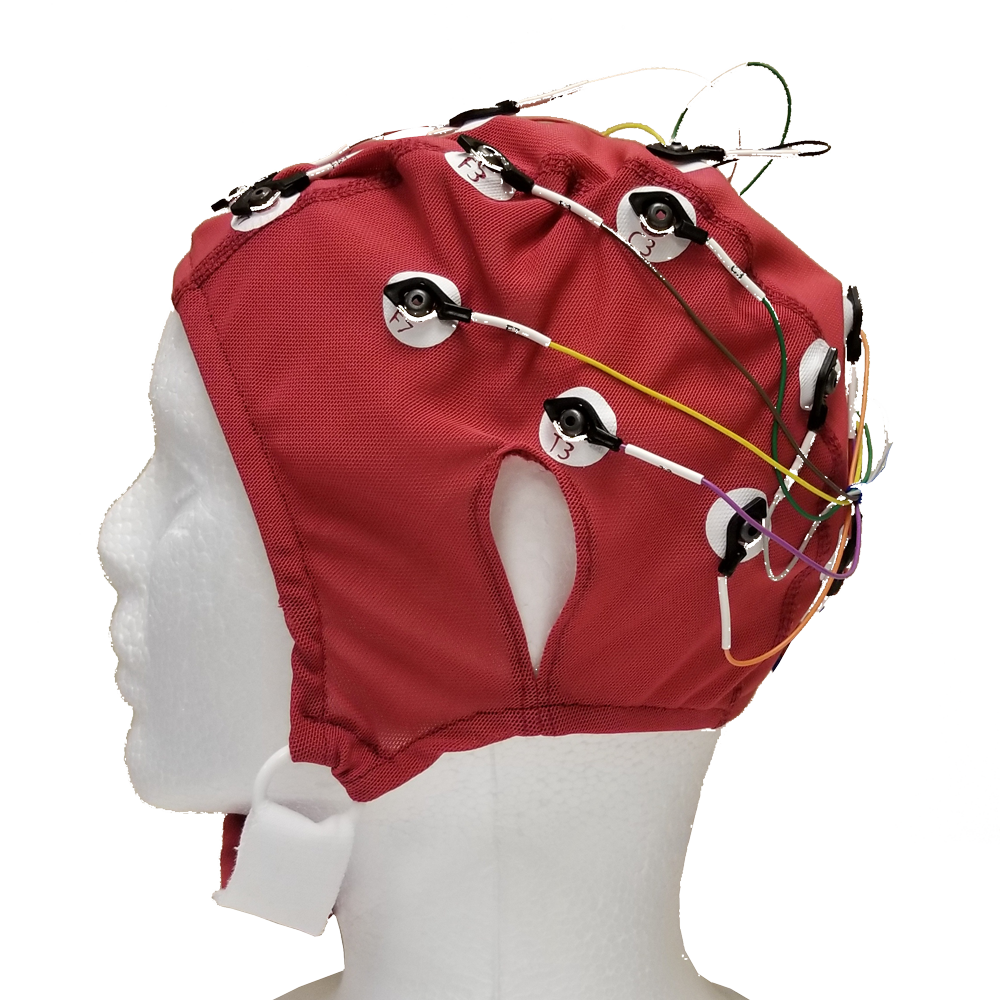
\includegraphics[width=0.3\textwidth]{images/19E.png}
        \caption{An example of tool to record the brain electrical signal}
    \end{figure} 
    
    \subsection{Electroencephalography}
    
     EEG is an method to record the neural oscillations of the brain and illustrate the operation of the body of human by that electrical signals. A different region of the brain and a different of body's activity produce a different type of EEG signal. Thus, in almost any scenario of recording EEG, one recorder cannot illustrate the whole status of the brain, but we have to create a matrix of multiple electrodes to record multiple zone in the brain. Each place in the head will generate a different signal and to be more specific, the electrode map has been normalized and use seamlessly all around the world. Furthermore, each recorder has it's own name in order to specify the region that it records. 
    
   
    
    The human brain divide into 5 main sections, and each has a specific roll to control the body both physical and mental:
    
    \begin{itemize}
        \item Frontal lobe (F) (Red)
        \item Cerebellum (C) (Cyan)
        \item Parietal lobe (P) (Yellow)
        \item Occipital lobe (O) (Emerald)
        \item Temporal lobe (T) (Green)
    \end{itemize}
    
    \begin{figure}[h]
        \centering
        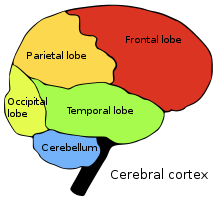
\includegraphics[width = 0.3\textwidth]{images/Brain.png}  
        \caption{Region of the brain}
        \label{fig:region_of_the_brain}
    \end{figure}
    
    Each of these regions produce different signal and if there is any skew on the place to set the electrode, it will have the wrong result. The figure below show the name and the places to put electrode on the skull. As you can see, figure 2.3 illustrates the full scale of electrode map. However, to simplify this case, The number of electrodes that we use can also can be reduced to 19 electrodes map as the figure 2.4.

    \begin{figure}
    \centering
    \begin{minipage}{.5\textwidth}
      \centering
      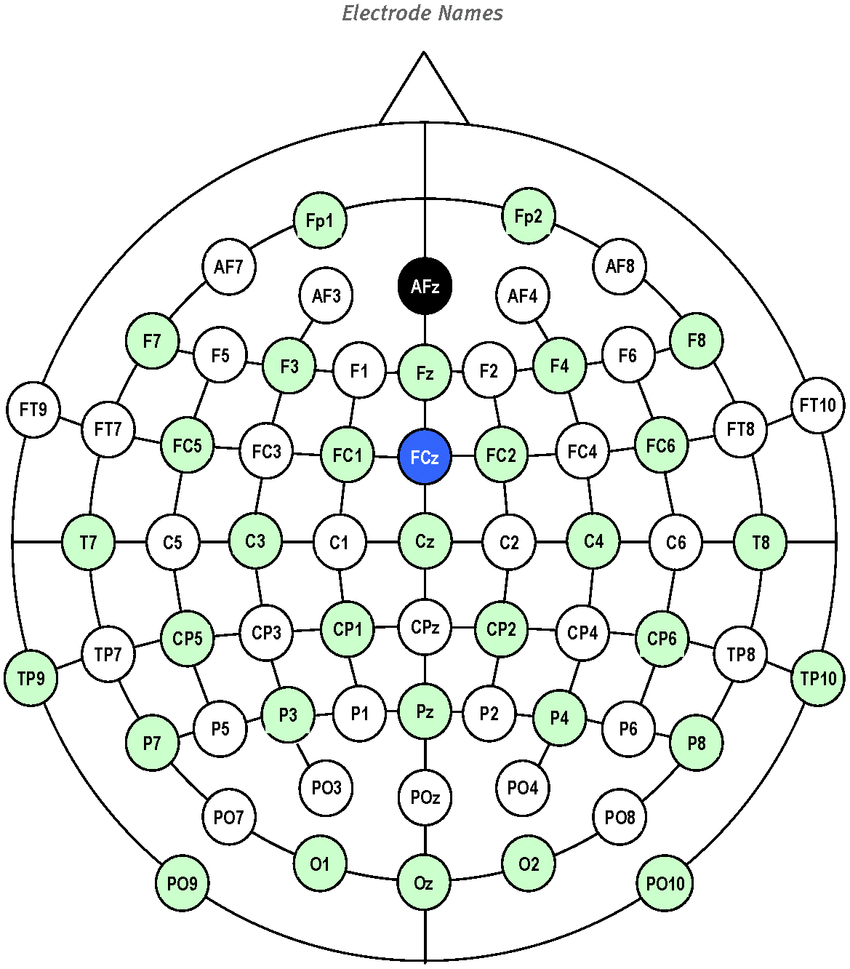
\includegraphics[width=.6\linewidth]{images/EEG_electrodes_map_full.png}
      \captionof{figure}{Full electrode map}
      \label{fig:fulle}
    \end{minipage}%
    \begin{minipage}{.5\textwidth}
      \centering
      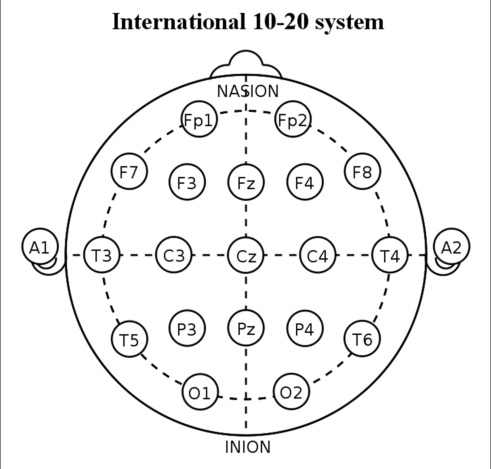
\includegraphics[width=.7\linewidth]{images/EEG_electrodes_map_19.png}
      \captionof{figure}{19 electrodes map}
      \label{fig:19e}
    \end{minipage}
    \end{figure}

    Electrode when recording the EEG signal it is contained not just only the signal, but also the noise from an extremely noisy environment. Only very tiny electric field or other electronic devices can affect how the recording process of electrode. Beside the noise come from the recording equipment itself and equipment from the surrounding area, Inside human body, some of the organ also generate electrical signal and it affects the final result. The most significant example of the organs that also create electric is our heart and our eyes. Heart beats and blinking also affect the EEG signal. Electrocardiography( heart signal) and electrooculography ( eyes signal) is the name of these two.

    The figure below demonstrates a typical 19-electrode system. As you can see, in each point of the electrode, the signal tends to be oscillate over an average line. But with the noise include, there is places that peak and not arrange in the average line and we need to get rid of them. We need a good filter to remove the noise otherwise it will make a bad approach to final data before apply machine learning technique in the signal.

    \begin{figure}[h]
        \centering
        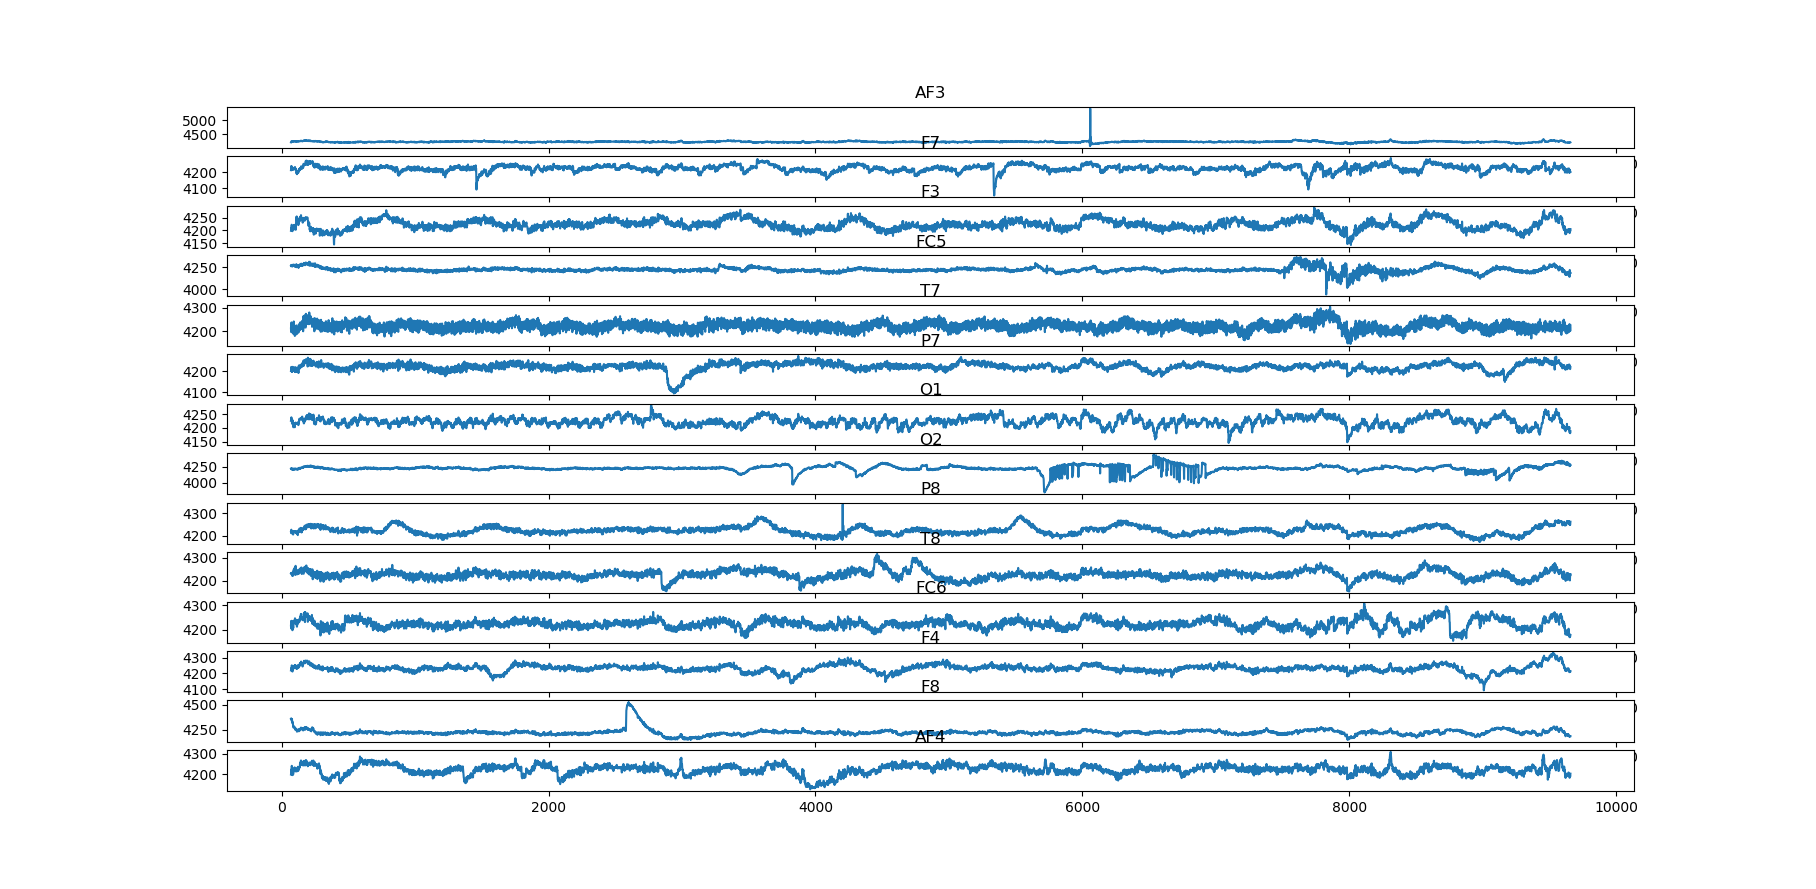
\includegraphics[width=1\textwidth]{images/EEGExample.png}
        \caption{Example of a typical EEG signals}
    \end{figure} 
    
\section{Apply machine learning in EEG signal}
    There are several types of machine learning to process the signal after all the noise be cleaned. For example, people can use neural network, Bayesian classifier, clustering and more. Even before applying machine learning method in the data we have, to be more accurate, It is also can use some technique to reduce the nodes by using nature-inspired algorithms like Genetic Algorithms (GA) and Simulating Annealing (SA)~\cite{EEG}. However, in this article, I will focus on using neural network to map the region of the brain we have with specific brain signal.
    
    It is important to know that the signal we have belong to the what part of the brain. So in this thesis I will focus using neural network to classify the 4 main region as I have cite in the subsection 1.1.2. Region P and O are very close so I will make it 1 class.
    
    \begin{itemize}
        \item Class 1: Frontal lobe (F)
        \item Class 2: Cerebellum (C)
        \item Class 3: Temporal lobe (T)
        \item Class 4: Parietal lobe (P) and Occipital lobe (O)
    \end{itemize}    
    
    \begin{figure}[h]
        \centering
        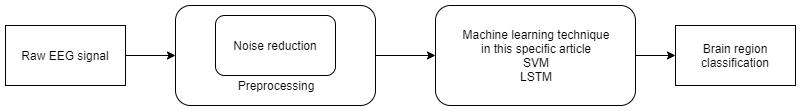
\includegraphics[width=1\textwidth]{images/GeneralDiagram.png}
        \caption{General diagram of a signal based region classification system.}
    \end{figure}
    
    The figure above illustrates the process that we will use to make the Raw EEG signal to the output is the classes mapping with the brain regions that we listed before.

\chapter{Materials}
\section{Tools}
    Python is an interpreted, high-level programming language. Python is an object-oriented programming language and really dynamic and flexible. It is believe that python is a minimalistic language. Developer can really focus on the real issue, not its syntax~\cite{GGGG}. Further more, Python is used too solve the problem in this article is because the variety in library. Python support very good in process large amount of data.
    
    Beside amazing feature that come original from Python, Python also support the tools and famous library that widely use in machine learning and more specific in this case is recursive neural network. In this thesis, I will use scipy for denoising the signal and keras to make a recursive neural network.

    \subsection{MNE-python}
    MNE is a very powerful tool to exploring, visualizing, and analyzing human neurophysiological data: MEG, EEG, sEEG, ECoG, and more. Most of the tool in this Python application we will not use, but to simplify the process of visualize signal before and after we apply filter, this tool is very convenient. MNE-tool tends to be a great library in this major, but in this article, we will not use the available preprocessing tools that available in the tools, but only use it to visualize the input and also the preprocessed signal before we do any further process~\cite{MNE}.
    
    \subsection{Keras}
    Most of the deep learning library in the market right now receive supports by some large companies. For example Facebook has Pytorch and Caffe2 or Microsoft has CNTK. However, we will use the most famous library from Google, whichs is Keras base on Tensorflow.
    
    The figure below illustrates the market share of Tensorflow and Keras from Google\cite{marketshare}. As you can see in the figure 2.1, Tensorflow and Keras have very large amount of user than any other libraries because of the simplicity that the tool bring to us. Thus, We will use Keras as the high-level library with the low-level is Tensorflow to make it simple. Keras has much simple syntax than Tensorflow itself.
    
    \begin{figure}[h]
        \centering
        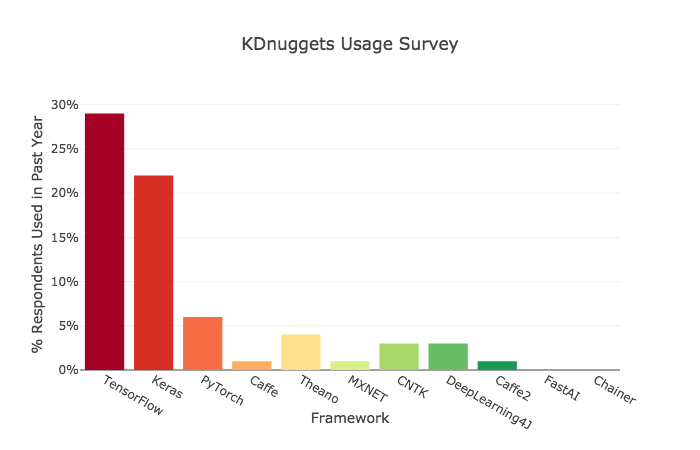
\includegraphics[width = 0.9\textwidth]{images/KERA_usage.png} 
        \caption{KDnuggets usage survey}
        \label{fig:marketshare}
    \end{figure}
    
    \subsection{Some famous python library}
    Pandas, Numpy and Matplotlib are very famous libraries in Python. We could say that these libraries are buildings the fundamentals of the successful that the reason we use Python for. Beside of the fundamental library, for this specific article, The list below show some more of the library that we will use in this problem.
    
    \begin{itemize}
        \item Scipy
        
        In this article, we will use Scipy for caculate the Z-score of the datasets, and use Z-score as a outliers detection in order to remove these artifact that appeared in the signal.
        \item Random
        
        The random library is used to mix the labeled data that we feed to the neural network. If we do not mix the divided dataset with each others, it is believe that the model is not so good in learning things from the signal we have.
        \item Pickle
        
        After we have the preprocessed data complete, We do not want to run that every time we use the processed signal again, so Pickle will export the data we processed to a file for later usage.
        \item Scikit learn
        
        The Scikit learn library does a important roll to normalize the signal which is raise the learning rate.
    \end{itemize}
    
\section{Datasets}
    The data I use in this article was provide by professor Sebastian Basterrech. The dataset contains 19 different electrodes, which is FP1-AVE,FP2-AVE, F3-AVE, F4-AVE, C3-AVE,  C4-AVE, P3-AVE, P4-AVE, O1-AVE,  O2-AVE, F7-AVE, F8-AVE, T3-AVE, T4-AVE, T5-AVE, T6-AVE, Fz-AVE, Cz-AVE and Pz-AVE. Each electrode have a specific position in the head, and the name represent its location. The number of electrode is the 10-20 international electrode system.
    
    This version has been reduced compare to the full electrode version. If we put too much electrode to record the electrical signal, It will be have intersections between electrodes and the output results might not so correct to determine which electrode is belong to which region of the brain.
    
    There are also almost 17000 data point, so to display all the data I use is impossible. The figure below only represent 15 first line of the data we use in this article. I can show this short version by using head\(\) function built-in in pandas. The first data point will be in zero for more equal between electrodes.

    \begin{figure}[h]
        \centering
        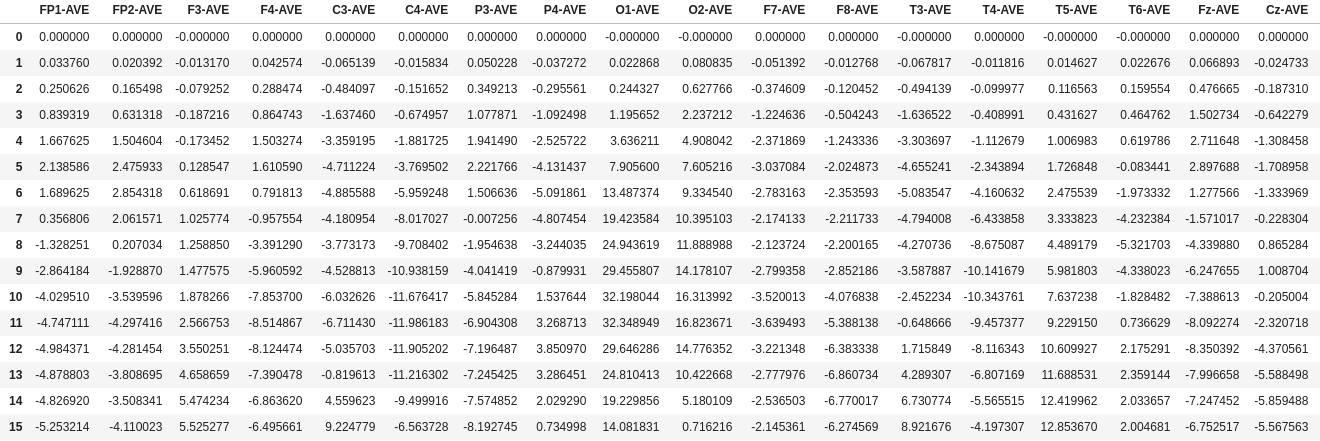
\includegraphics[width=1\textwidth]{images/data.png}
        \caption{First 15 data points}
    \end{figure}

    You can see more details the place that these electrodes sit on the skull in order to know the location of the name of the electrodes in chapter 1. The electrode is divided into 4 classes as we discussed before. The first character of the name contain the location that the electrode measure.
    
    \begin{itemize}
        \item Class 0: Frontal lobe (F) 
        
        including FP1-AVE, FP2-AVE, F3-AVE, F4-AVE, F7-AVE, F8-AVE, Fz-AVE
        \item Class 1: Cerebellum (C) 
        
        including C3-AVE, C4-AVE, Cz-AVE
        \item Class 2: Temporal lobe (T) 
        
        including T3-AVE, T4-AVE, T5-AVE, T6-AVE
        \item Class 3: Parietal lobe (P) and Occipital lobe (O) 
        
        including P3-AVE, P4-AVE, Pz-AVE, O1-AVE,  O2-AVE
    \end{itemize}
    
    
 
\chapter{EEG pre-processing}
\section{Visualize EEG signals}
    To have a nice overview between the dataset before and after remove noise, we should visualize the signal the signal first. We can also visualize the dataset with traditional tool like Matplotlib. However, Matplotlib basically just draw the dataset. Fortunately, MNE-Python is a powerful tool help us to mark the bad-channels, interact with the signal and a easier look at the very first before we apply any filter as well as afterward. 
    
    MNE-Python supports a lot of digital formats of EEG signal but the format that we have is not available in library. However, MNE give us the option to create the "raw" MNE signal file from scratch with other file format such as .csv or .tdt. First, we have to create a basic information about the structure of the signal we about to input. We have 19 electrodes so according to that, we have 19 members in the channel names.
    
    \begin{lstlisting}
        channel_names = ['FP1', 'FP2', 'F3', 'F4', 'C3', 'C4', 'P3', 'P4', 'O1', 'O2', 'F7', 'F8', 'T3', 'T4', 'T5', 'T6', 'Fz', 'Cz', 'Pz']
        sfreq = 240
        info = mne.create_info(channel_names, sfreq) 
    \end{lstlisting}
    
    In here, we have the information of the name of all electrodes that we have with the frequency of 240Hz. after import the basic information as well as the data itself we now can create the raw data of the signal with the EEGsignalValues is the data.
    
    \begin{lstlisting}
    raw = mne.io.RawArray(EEGsignalValues, info)
    \end{lstlisting}
    
    \begin{figure}
    \centering
    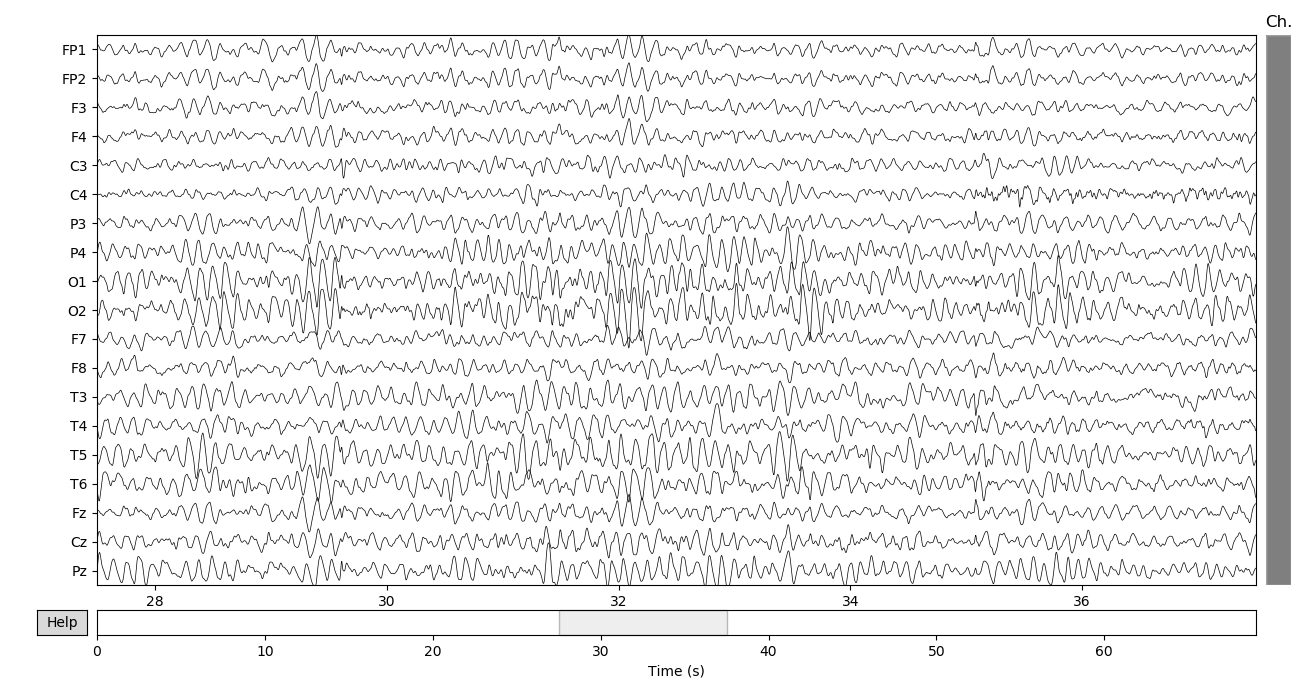
\includegraphics[width = 0.9\textwidth]{images/EEG_with_MNE.png}
    \caption{Visual EEG signal with MNE-python}
    \label{fig:visualEEGwithMNE}
    \end{figure}
    
    The result of the MNE-tool is shown in the figure 3.1. In here, we have the information of the name of all electrodes that we have with the frequency of 240Hz. after import the basic information as well as the data itself we now can create the raw data of the signal.
    
\section{Noise reduction}
    There are a lot of technique can be apply on the raw signal to remove the outliers that exist in our data. We have some of the very famous technique. The EEG signal only contain some of the frequency, and any signal that below that or above that should be remove from the signal. 
    We can deal with it by apply high-pass filter and low-pass filter. However, in our specific datasets, we will use a popular method to detect and remove outliers and it is called Z-score outliers detection.
    
    Z-score is a numerical measurement, indicates how many standard deviations an element is from the mean\cite{z_score}. The formular to caculate the score is below.

    $$z={{x-\mu}  \over \sigma }$$
    
    % $$\mid x\lfloor \sigma \rfloor \lfloor k \rfloor - \mu \lfloor k \rfloor\mid < \mid \alpha\delta^2 \mid$$

    The bigger the score is, the further the point is compare with the mean of the whole data set. If the Z-score of a point consider far enough from the mean, it is considered as an outlier. In this case, I want to consider around 5 percent of the signal as artifacts. Thus, any data point that have the Z-score over 3 and less than -3 will be removed from signal.
    
    \begin{figure}[h]
        \centering
        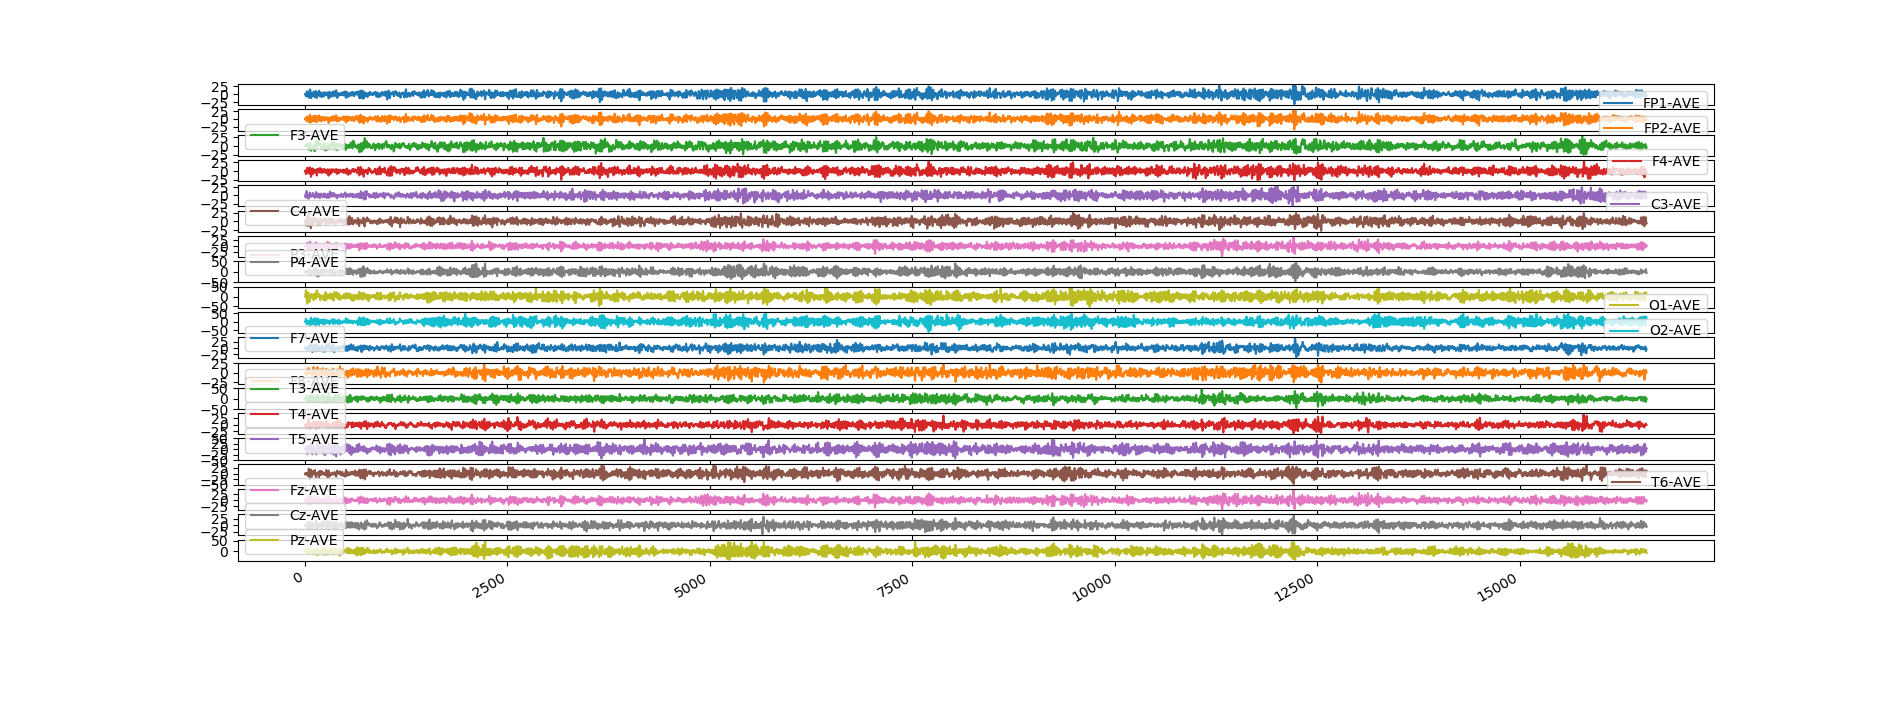
\includegraphics[width = 0.7\textwidth]{images/OriginalData.png}
        \caption{Original data}
        \label{fig:original_data}
    \end{figure}
    
    Figure~\ref{fig:original_data} is the visualized data of the signal before any impact. However, this is too small to show any changes has been made by the filter so we will only focus on a example of the FP1 signal. On the figure~\ref{fig:compare} is the electrode FP1 only. You can notice that there is some changes that applied here.
    
    \begin{itemize}
    \item Blue line: before apply Z-score
    \item Orange line: after apply Z-score
    \end{itemize}
    
    \begin{figure}[h]
        \centering
        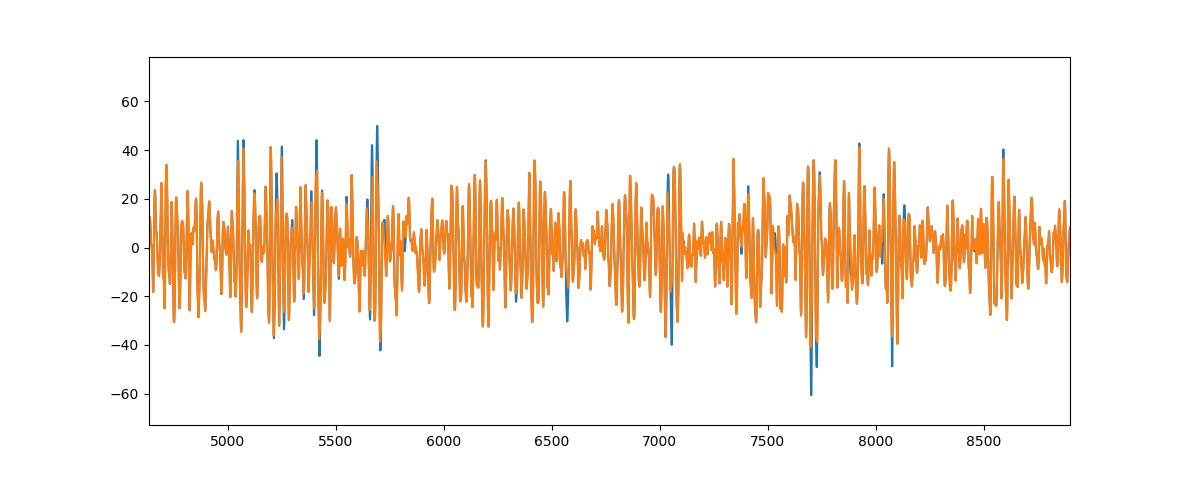
\includegraphics[width = 1\textwidth]{images/fp1-2.png}
        \caption{A part of FP1 before and after apply Z-score}
        \label{fig:compare}
    \end{figure}
    
    More closer look.
    
    \begin{figure}[h]
        \centering
        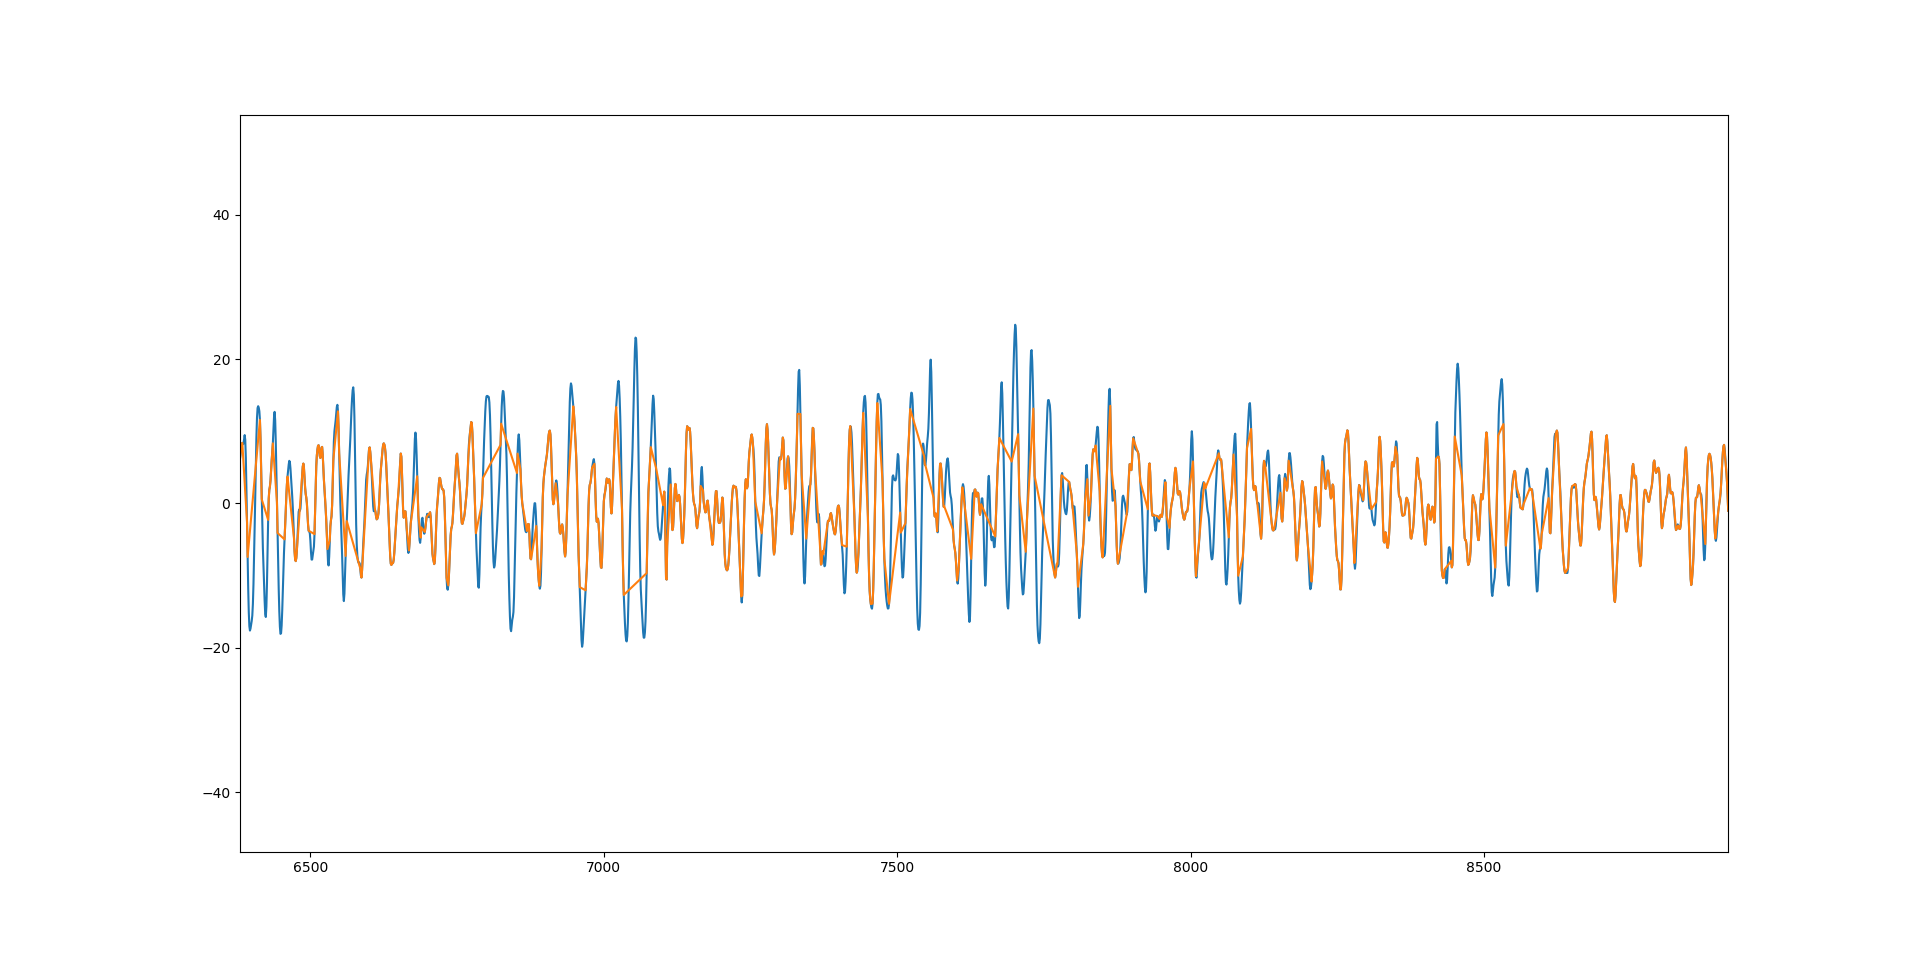
\includegraphics[width = 1\textwidth]{images/closer.png}
        \caption{Closer look at signal recorded by the electrode FP1 }
        \label{fig:closer}
    \end{figure}
    
    You can see that there is some boundary has been made all over the signal. the removed outliers around 5.7 percent of the dataset. This technique to reduce noise in the data is still not wipe all the noise but it is the most efficient technique.
    
    In the future, we can do some research about how to remove other artifact that is very hard to remove and cannot do this by normal filter. That is EOG signal and ECG signal, affected when we blinking or when our heart beating.

\chapter{Machine learning methods}
\section{Learning set creation}
    \subsection{Table creation}
        We now have a denoised dataset 19 column table. Our mission now to unroll it in to a long table with 2 columns, the first one is the name of the electrode and the others is the value. The melt function is used to do this. We change the variable to match the class from 0 to 3 as below:
        
        \begin{itemize}
        \item Class 0: including FP1-AVE, FP2-AVE, F3-AVE, F4-AVE, F7-AVE, F8-AVE, Fz-AVE
        \item Class 1: including C3-AVE, C4-AVE, Cz-AVE
        \item Class 2: including T3-AVE, T4-AVE, T5-AVE, T6-AVE
        \item Class 3: including P3-AVE, P4-AVE, Pz-AVE, O1-AVE,  O2-AVE
    \end{itemize}

        \begin{figure}[h]
        \centering
        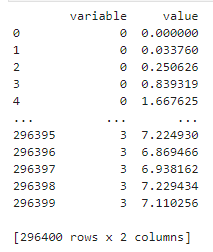
\includegraphics[width = 0.3\textwidth]{images/unroll.png}
        \caption{Unrolled dataset}
        \label{fig:unroll}
        \end{figure}
        
        Figure~\ref{fig:unroll} illustrate a part of the signal after unroll the signal. The first column will be variable, which is indicates the class of the data step. The second column indicates the value of the data steps itself.
      
      In this specific article, This dataset will be divide into multiple time window frame W with multiple data steps in order to create multiple data points so we can apply machine learning method. We will test in 2 type of time windows W to see if there is any difference.
      
      \begin{itemize}
          \item Time window W1: 200 steps each
          \item Time window W2: 400 steps each
      \end{itemize}
      
      \subsection{Shuffling}
        To make the data reduce variance and making sure the model general and less over fit, We will need to shuffle the data before do any further. Fortunately, python has built-in a random library and it make us more easy.
        
        \begin{lstlisting}
        import random
        random.shuffle(training_data)
        \end{lstlisting}
        
        With time windows W1, we have 1482 data points and with time windows W2, we have 741 data points. I will separate around 20\% of the dataset we have here to create a testing set, and the other 80\% will be training set. Thus, W1 have 1282 points in training set and 200 points in testing set, and the others W2 will be 641 for training and 100 for testing.
            
\section{Apply machine learning}
    In order to find the best machine learning method that we should apply in specify the region of the brain, I want to use 2 method here. The first is long short-term memory recursive neural network and the other is super vector machine.
    \subsection{LSTM-RNN}
    Our brain do not start from scratch every it processes. When you read this thesis, you understanding base on your knowledge and previous words. We do not throw everything and start again. But the traditional neural network cannot do this. However, recursive neural network can do this. It has loop in the network and allow the information that the network learnt to persist. Figure~\ref{fig:RNN} demonstrates a RNN network.
    
    Thus, there is still a problem with RNN. The network tends to "forget" what it has learnt long ago in the previous. Long short-term memory networks, for short is LSTMs, are a special kind of RNN, and it has ability to learn long-term dependencies~\cite{NeuralNetwork}. They were introduced first time by Hochreiter \& Schmidhuber in 1997, and now is a very famous and widely use. LSTM works really well in a large scale problem. It is design for long-term dependency, and remember things it is natural with LSTM, not forced it to learn~\cite{LSTM}.
    
    \begin{figure}[h]
        \centering
        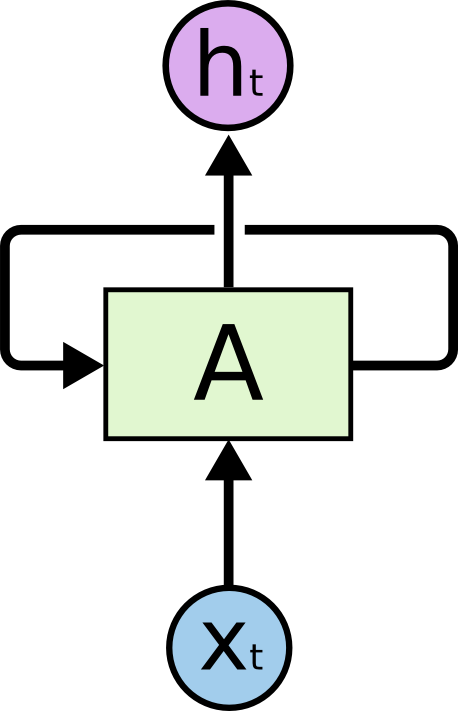
\includegraphics[width = 0.2\textwidth]{images/RNN-rolled.png}
        \caption{RNN-rolled}
        \label{fig:RNN}
    \end{figure}
    
        \begin{lstlisting}
    model = Sequential()

    model.add(LSTM(16, input_shape=(X.shape[1:]), activation='relu', return_sequences=True))
    model.add(Dropout(0.2))
    
    model.add(LSTM(16, activation='relu'))
    model.add(Dropout(0.2))
    
    model.add(Dense(10, activation='relu'))
    model.add(Dropout(0.2))
    
    model.add(Dense(4, activation='softmax'))
    
    opt = tf.keras.optimizers.Adam(lr=0.001, decay=1e-6)
    
    # Compile model
    model.compile(
        loss='sparse_categorical_crossentropy',
        optimizer=opt,
        metrics=['accuracy'],
    )
    \end{lstlisting}
    
    In this article, I will create a 4 layers neural network. First 2 layers is LSTM with 16 cells each and activation layer is rectifier linear unit. The next layer is a dense layer with 10 units. Finally, the output layer has 4 units corresponding to 4 output class that we have discussed before. The figure~\ref{fig:LSTMDiagram} will visualize the structure of this network. We will feed this network with both the dataset with W1 and W2 data to have a nice comparison and see which is the most accurate when apply LSTM.
    

    \begin{figure}[h]
        \centering
        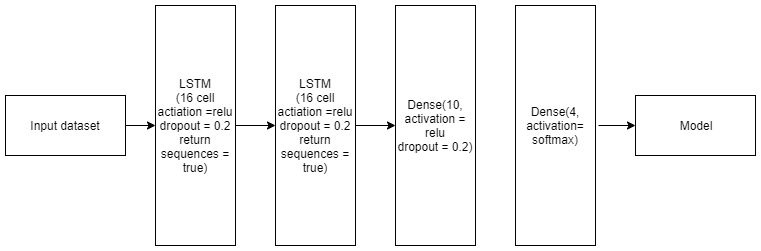
\includegraphics[width = 1\textwidth]{images/LSTMDiagram.png}
        \caption{Neural network breakdown diagram}
        \label{fig:LSTMDiagram}
    \end{figure}
    
    
    \subsection{SVM}
    
     SVM is a very popular supervised machine learning models that from the input data users give do classification and regression. With input data already labeled, the output of SVM is an optimal hyper plane which categorizes new data points~\cite{GG}. For example, in 2D space, hyper plane is a line create the boundary between 2 groups of data. SVM also can work well in multidimensional. 
    
    Scikit learn have already built-in the SVM function and we can easily implement this function. I will use SVC with gamma value is scale for better result. We also will separate 20\% of the dataset we have to create a validate set to check of accuracy of the model. I will leave the default kernel of SVC is radial basis function~\cite{GGG}.

\chapter{Empirical results}
The electrode system that we use to measure is really sensitive. The advantage of this is that we can measure the small signal from the brain, but it comes along side with disadvantage. The surrounding environment with electrical field can impact the recorded EEG signal, so that it makes the accuracy lower. With Z-score, we have not removed all the possible outliers.

\section{LSTM RNN}

\begin{table}[h]
\centering
\begin{tabular}{|l|l|l|}
\hline
          & W2 = 400                        & W1 =200                         \\ \hline
Epoch 1/2 & acc = 0.3173, val\_acc = 0.4255 & acc = 0.1941, val\_acc = 0.2626 \\ \hline
Epoch 2/2 & acc = 0.3387, val\_acc = 0.4326 & acc = 0.2662, val\_acc = 0.3805 \\ \hline
\end{tabular}
\caption{Accuracy using LSTM with windows W1=200 and W2=400 time steps}
\label{table:LSTM}
\end{table}

The table~\ref{table:LSTM} demonstrates the accuracy when we apply LSTM on the dataset. In this 2 cases, we can clearly see that the accuracy  of the case W2 is higher than case W1, when we divide the windows W2 times larges. The system with windows W2 have a slightly more accuracy than case W1, with 0.4182 in the validation set in W1 and 0.3805 in case W2. 

\section{SVM}

\begin{table}[h]
\centering
\begin{tabular}{|l|l|}
\hline
W2 = 400        & W1 =200          \\ \hline
accuracy = 0.72 & accuracy = 0.575 \\ \hline
\end{tabular}
\caption{Accuracy using SVM with windows W1=200 and W2=400 time steps}
\label{table:SVM}
\end{table}

The table~\ref{table:SVM} indicates the results of the accuracy when classify the brain region using SVM. As you can see, just like in RNN, the windows W2 case have a better accuracy when i validate on a separate dataset with 0.2 of the original dataset. The accuracy is 0.72 compare to only 0.575 on the set with windows W1. 

% \begin{figure}
%      \centering
%      \begin{subfigure}[b]{0.3\textwidth}
%          \centering
%          
\includegraphics[width=\textwidth]{logo2}
%          \caption{$y=x$}
%          \label{fig:y equals x}
%      \end{subfigure}
%      \hfill
%      \begin{subfigure}[b]{0.3\textwidth}
%          \centering
%          
\includegraphics[width=\textwidth]{logo2}
%          \caption{$y=3sinx$}
%          \label{fig:three sin x}
%      \end{subfigure}
%      \hfill
%      \begin{subfigure}[b]{0.3\textwidth}
%          \centering
%          
\includegraphics[width=\textwidth]{logo2}
%          \caption{$y=5/x$}
%          \label{fig:five over x}
%      \end{subfigure}
%         \caption{Three simple graphs}
%         \label{fig:three graphs}
% \end{figure}

\chapter{Conclusion and future works}
\section{Conclusion}

With the results we have, it is clearly seen that the best accuracy for brain region classification is SVM machine learning algorithm. With LSTM, it is seen that it is not a good technique in this specific problem, with the accuracy of SVM in W2 is 0.72, which is pretty accurate compared to only 0.42 on LSTM, and it makes it not usable. The second thing that we see is that with time windows equal 400 time steps it is more accurate than 200. I can only divide the maximum dataset to 400 time steps per window, otherwise it will be lack of sample. This reason is because I have a lack of data and it will be more difficult. I think it will be more accurate if we have more data. This study if it successes can bring benefits for analyzing the plasticity of the brain as well as understanding how the damaged brain provokes changes in their functionality. 

\section{Future works}
According to our experiments, the highest accuracy was 72\%. Therefore, It is still possibilities of improving the classifier. We figured out that some of these reasons might affect the result and there are still works to solve in the future:

\begin{enumerate}
    \item Lack of data:
    
            The data we have is still not enough. We only have around 1400 data points with the case W1 and around 700 with case W2. Thus, this problem impacts the result we have.
    \item Still have noise:
    
            What we have done to denoise by using Z-score is only removing the significant artifact is made by the equipment or the environment. We still have not removed ECG and EOG from the dataset we have. In the future, the classification can be more accurate by getting rid of them.
            
            High-pass and low-pass filter also can be applied to remove the noise and make it more accurate.
\end{enumerate}

In the future, we need to collect more data and have to work more on removing outliers in order to have a better result.

\appendix
\chapter{Setup the environment}
All of the setup below is done inside Linux environment. You can find tutorial for Windows and other platform in website https://www.anaconda.com.

Step 1: Download Anaconda script
\begin{lstlisting}
cd /tmp
curl -O https://repo.anaconda.com/archive/Anaconda3-2019.03-Linux-x86_64.sh
\end{lstlisting}

\bigskip
Step 2: Run the Anaconda script
\begin{lstlisting}
bash Anaconda3-2019.03-Linux-x86_64.sh
\end{lstlisting}
You will receive the following output to review the license agreement by pressing ENTER until you reach the end.
\begin{lstlisting}
Welcome to Anaconda3 2019.03

In order to continue the installation process, please review the license
agreement.
Please, press ENTER to continue
>>>
...
Do you approve the license terms? [yes|no]
\end{lstlisting}
Type yes to agree with the license.
Now you have done with installing python.

\bigskip
Step 3: Install dependency
\begin{lstlisting}
conda install -c anaconda numpy
conda install -c anaconda pandas
conda install -c anaconda matplotlib
conda install -c conda-forge mne
conda install -c conda-forge keras
\end{lstlisting}
After done all the steps above, the system is good to go if you are ok using notepad to code python. But VSCode or Jupyter lab is a extremely good replacement with supported tools, for example, IntelliSense for auto complete the code.
\begin{lstlisting}
conda install -c conda-forge jupyterlab
\end{lstlisting}
With the VSCode, you have to add a repository.
\begin{lstlisting}
sudo apt updatesudo apt install software-properties-common apt-transport-https wget
wget -q https://packages.microsoft.com/keys/microsoft.asc -O- | sudo apt-key add -
sudo add-apt-repository "deb [arch=amd64] https://packages.microsoft.com/repos/vscode stable main"
sudo apt updatesudo apt install code
\end{lstlisting}
And you good to go.

\chapter{Medical use of EEG~\cite{Medical}}
EEG is one of the main diagnostic tests for epilepsy. A routine clinical EEG recording typically lasts 20–30 minutes (plus preparation time). It is a test that detects electrical activity in your brain using small, metal discs (electrodes) attached to your scalp. Routinely, EEG is used in clinical circumstances to determine changes in brain activity that might be useful in diagnosing brain disorders, especially epilepsy or another seizure disorder. An EEG might also be helpful for diagnosing or treating the following disorders:
\begin{itemize}
    \item Brain tumor
    \item Brain damage from head injury
    \item Brain dysfunction that can have a variety of causes (encephalopathy)
    \item Inflammation of the brain (encephalitis)
    \item Stroke
    \item Sleep disorders
\end{itemize}

It can also:
\begin{itemize}
    \item distinguish epileptic seizures from other types of spells, such as psychogenic non-epileptic seizures, syncope (fainting), sub-cortical movement disorders and migraine variants.
    \item differentiate "organic" encephalopathy or delirium from primary psychiatric syndromes such as catatonia.
    \item serve as an adjunct test of brain death in comatose patients.
    \item prognosticate in comatose patients (in certain instances).
    \item determine whether to wean anti-epileptic medications.
\end{itemize}

At times, a routine EEG is not sufficient to establish the diagnosis and/or to determine the best course of action in terms of treatment. In this case, attempts may be made to record an EEG while a seizure is occurring. This is known as an ictal recording, as opposed to an inter-ictal recording which refers to the EEG recording between seizures. To obtain an ictal recording, a prolonged EEG is typically performed accompanied by a time-synchronized video and audio recording. This can be done either as an outpatient (at home) or during a hospital admission, preferably to an Epilepsy Monitoring Unit (EMU) with nurses and other personnel trained in the care of patients with seizures. Outpatient ambulatory video EEGs typically last one to three days. An admission to an Epilepsy Monitoring Unit typically lasts several days but may last for a week or longer. While in the hospital, seizure medications are usually withdrawn to increase the odds that a seizure will occur during admission. For reasons of safety, medications are not withdrawn during an EEG outside of the hospital. Ambulatory video EEGs therefore have the advantage of convenience and are less expensive than a hospital admission, but the disadvantage of a decreased probability of recording a clinical event.

Epilepsy monitoring is typically done to distinguish epileptic seizures from other types of spells, such as psychogenic non-epileptic seizures, syncope (fainting), sub-cortical movement disorders and migraine variants, to characterize seizures for the purposes of treatment, and to localize the region of brain from which a seizure originates for work-up of possible seizure surgery.

Additionally, EEG may be used to monitor the depth of anesthesia, as an indirect indicator of cerebral perfusion in carotid endarterectomy, or to monitor amobarbital effect during the Wada test.

EEG can also be used in intensive care units for brain function monitoring to monitor for non-convulsive seizures/non-convulsive status epilepticus, to monitor the effect of sedative/anesthesia in patients in medically induced coma (for treatment of refractory seizures or increased intracranial pressure), and to monitor for secondary brain damage in conditions such as subarachnoid hemorrhage (currently a research method).

If a patient with epilepsy is being considered for resective surgery, it is often necessary to localize the focus (source) of the epileptic brain activity with a resolution greater than what is provided by scalp EEG. This is because the cerebrospinal fluid, skull and scalp smear the electrical potentials recorded by scalp EEG. In these cases, neurosurgeons typically implant strips and grids of electrodes (or penetrating depth electrodes) under the dura mater, through either a craniotomy or a burr hole. The recording of these signals is referred to as electrocorticography (ECoG), subdural EEG (sdEEG) or intracranial EEG (icEEG)--all terms for the same thing. The signal recorded from ECoG is on a different scale of activity than the brain activity recorded from scalp EEG. Low voltage, high frequency components that cannot be seen easily (or at all) in scalp EEG can be seen clearly in ECoG. Further, smaller electrodes (which cover a smaller parcel of brain surface) allow even lower voltage, faster components of brain activity to be seen. Some clinical sites record from penetrating microelectrodes.

Recent studies using machine learning techniques such as neural networks with statistical temporal features extracted from frontal lobe EEG brainwave data has shown high levels of success in classifying mental states (Relaxed, Neutral, Concentrating), mental emotional states (Negative, Neutral, Positive) and thalamocortical dysrhythmia.

EEG is not indicated for diagnosing headache. Recurring headache is a common pain problem, and this procedure is sometimes used in a search for a diagnosis, but it has no advantage over routine clinical evaluation.

%\printbibliography
%\printbibliography
\bibliographystyle{abbrv}
\bibliography{References}

\end{document}